\documentclass[10pt,a4paper]{article}
\usepackage[utf8]{inputenc}
\usepackage{amsmath}
\usepackage{amsfonts}
\usepackage{mathtools}
\usepackage{amssymb}
\usepackage{graphicx}
\usepackage{subcaption}
\usepackage{dsfont}
\usepackage[strict]{changepage}
\usepackage{float}
\usepackage{parskip}
\makeatletter
\newcommand*{\transpose}{%
  {\mathpalette\@transpose{}}%
}
\newcommand*{\@transpose}[2]{%
  % #1: math style
  % #2: unused
  \raisebox{\depth}{$\m@th#1\intercal$}%
}

\author{Adam Jalkemo \texttt{adam@jalkemo.se} \and
Alexander Israelsson \texttt{israelsson.alexander@gmail.com} \and
Emil Westenius \texttt{emil@westenius.se} \and
Jonathan Andersson \texttt{mat11ja1@student.lu.se}}
\title{Adaptive Friction Compensation}
\begin{document}
\maketitle

\section{Introduction}
In this project a Furuta pendulum process will be used. The Furuta pendulum consists of a pendulum, that is free to rotate in the vertical plane, attached to the end of an horizontally rotating arm that can be controlled. The pendulum will be stabilized in the inverted position using a swing up controller and a top controller. When controlling the pendulum in the top position limit cycles will occur due to friction. By compensating for the friction we aim to stabilize the pendulum, the friction will be estimated using an adaptive method. To do this a Java controller and interface will be implemented and run on a linux computer.
\section{Program structure}
For our suggested solution we will need one thread for the GUI and one for the controller. To communicate with the Furuta process we will use the analog box normally used during the control labs at LTH. The realtime package from Automatic Control at LTH will be used for communication in the GUI and controller implementation. It will be important to synchronize the controller calculations with the user inputs. A general overview can be seen in figure \ref{fig:uml}.
\begin{figure}[H]
\centerline{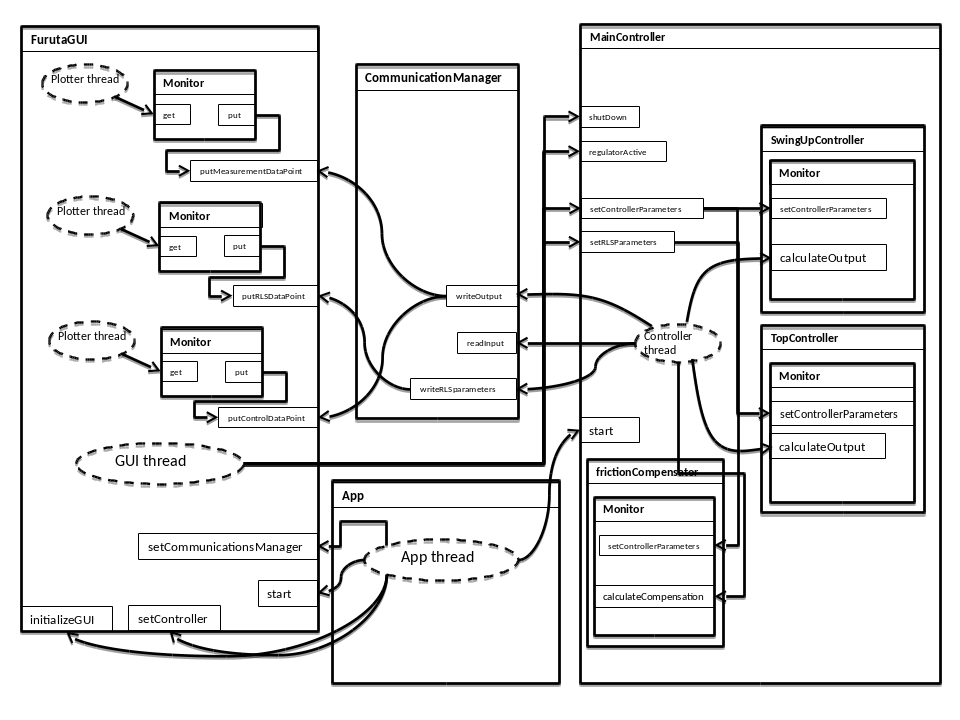
\includegraphics[scale=0.7]{notUml.png}}
\caption{Overview of the program structure}
\label{fig:uml}
\end{figure}
%% MORe STUFFS??

%ToDo UML AND DESCRIPTION OF CLASSES AND PACKAGES



%Todo what parameters can be changed.
\subsection{System model}
Due to the non-linear dynamics of the rotating arm and pendulum the modeling of the process becomes complicated. We have used the model given in Lab2 in "Non-linear control" where the model have been simplified with the help of Lagrange theory. The dynamics of the model is then given by:
$$(J_p + Ml^2)(\ddot{\theta} - \dot{\varphi} ^2\sin\theta \cos\theta )+Mrl\ddot{\varphi}\cos\theta-gl(M+m/2)\sin\theta = 0 $$
\begin{equation}
Mrl\ddot{\theta}\cos\theta - Mrl\dot{\theta ^2}\sin\theta + 2(J_p + ml^2 ) \dot{\theta} \dot{\varphi}\sin\theta \cos\theta + (J+mr^2 + Mr^2 + (J_p+ml^2)\sin^2\theta)\ddot{\varphi}=u
\label{eq:model}
\end{equation}
where $\theta$ is the angle of the pendulum, $\varphi$ is the angle of the arm and $u$ is the motor torque on the arm. The states $\theta$, $\dot{\theta}$, $\varphi$ and $\dot{\varphi}$ will all be measured from the process and $u$ will be our control signal. The approximated coefficients are also taken from Lab2 and are given by:
$$l=0.413m \quad  r=0.235m$$
$$M=0.01kg \quad J=0.05kgm^2$$
$$J_p=0.0009kgm^2 \quad m=0.02kg$$
$$ g=9.8$$
Where $l$ is the length of the pendulum, $r$ is the length of the arm, $M$ is the mass of the weight, $J$ is moment of inertia  for pendulum, $J_p$ is the moment of inertia for the arm, $m$ is the mass of the pendulum and $g$ is the gravity constant.
\subsubsection{Linearization}
Linearization of \ref{eq:model} is done around
\begin{equation}
x =
\begin{pmatrix}
\theta & \dot\theta & \varphi & \dot\varphi
\end{pmatrix} = 
\begin{pmatrix}
0 & 0 & 0 & 0
\end{pmatrix}
\end{equation}
which yields 
\begin{equation}
\dot{x} = Ax + Bu =
\begin{pmatrix}
0 & 1 & 0  & 0 \\
\frac{bd}{ab-c^2} & 0 & 0 & 0 \\
0 & 0 & 0 & 1 \\
\frac{-cd}{ab-c^2} & 0 & 0 & 0
\end{pmatrix}x
+
\begin{pmatrix}
0 \\
\frac{-cg}{ab-c^2} \\
0 \\
\frac{ag}{ab-c^2}
\end{pmatrix}u
\label{eq:linear}
\end{equation}
where 
$$ a = J_p + M l^2 \qquad b = J + M r^2 + m r^2 $$
$$ c = M r l  \qquad d = l g (M + m/2) $$
This corresponds to the arm fixed (at an angle corresponding to zero) with the pendulum fixed in the top position.
\subsubsection{Discretization}
The linearized model will be discretized. We would like to implement a way to change the sampling time online but this would require us to implement a function similar to $c2d$ in java. There are approximations that can be made so that we won't have to solve the integral over the matrix exponential but we need to be sure that the results are good enough. If we can't figure out a way to make a java implementation of $c2d$, we will discretize offline using matlab with the sample time $h=0.01$.
This yields
\begin{equation}
x_{k+1} = A_dx_k + B_du_k =\begin{pmatrix}
 1.0016 & 0.01 & 0 & 0 \\
 0.3133 & 1.0016 & 0 & 0 \\
 0 & 0 & 1 & 0.01 \\
 -0.0059 & 0 & 0 & 1 
\end{pmatrix}x_k + \begin{pmatrix}
-0.0036\\
-0.7127\\
 0.0096\\
 1.9125
 \end{pmatrix}u_k
 \label{eq:discrete}
\end{equation}

\subsection{Controller}
\subsubsection{Swing up}
For the swing up a Lyapunov based controller will be used. To do this we will use the total energy of the pendulum (kinetic and potential) given in \ref{eq:energy}.
\begin{equation}
E= Mgl(cos\theta - 1)+\frac{J_p}{2}\dot\theta^2
\label{eq:energy}
\end{equation}
We will use the Lyaponov candidate $V(x,a)=E^2$. Then by taking the derivative we aim to find a controller $a=F(x)$ which will make $\dot V \leq 0$ for all $x$. The controller will always output maximal control signal possible in order to minimize the Lyaponov function.
\subsubsection{Top controller}
In the top position a LQR controller will be used. To do this we will use the linearized model in eq. \ref{eq:linear} to calculate L. In order change the cost matrices Q and R online we must implement a way to calculate the state feedback gain vector L given by
$$ L = (R+B^TPB)^{-1}(B^TPA) $$
where P is calculated by iterating
$$ P_{k-1} = A^TP_kA-(A^TP_kB)(R+B^TP_kB)^{-1}(B^TP_kA)+Q $$
backwards in time with $P_N = Q$. This solution for the Riccati problem will not work for all systems but in this case Fredrik Bagge verified that it should work.

There are six measurement signal available for the controller to use. Two for the position $ \theta $ and velocity $ \dot{\theta} $ of the pendulum each (one has higher resolution and is used at the top position) and one for the arm position $ \varphi $ and velocity $ \dot{\varphi} $. The quality of signals is not known at the moment and we might need to use a Kalman filter.

\subsubsection{Controller switch}
In order to switch between the two controllers we need to find good conditions which enable the pendulum to be in a good position for when the top controller takes over. Since the model is linearized around 
$$x =
\begin{pmatrix}
\theta & \dot\theta & \varphi & \dot\varphi
\end{pmatrix} = 
\begin{pmatrix}
0 & 0 & 0 & 0
\end{pmatrix}$$
we need the pendulum to both have a low velocity and be close to the top for the top controller to work properly.
This will as of now done by one of two options. The first one is to form an ellipse from $\dot\theta$ and $\theta$ which will give good estimations of when to switch. The other option is to calculate the energy of the pendulum and cease all control signals when the proper amount of energy is reached in the pendulum. This will allow the pendulum to come to rest close to the top which will enable the top controller to take over easily. The second option is different from the first since we aim to use a certain time interval where no control signal is sent and therefor the pendulum will have a lower velocity when it reaches the proper position.
\subsubsection{Friction compensation}
After the friction has been estimated, see \ref{sec:fricEst}, the value of the friction in each time step will be added to the control signal. This will only be used in the top controller since the swing up controller will always output maximal control signal. When the pendulum is close to the top position we will need to add a dead-zone in order to keep the noise from the measurements from making the friction compensation add control signal in the wrong direction.

\subsection{Friction estimation}
\label{sec:fricEst}
To manage the friction we aim to estimate a simple friction model using RLS. The model will initially be a combination of Coulomb and viscous friction, i.e. the friction will be given by $$f=f_c\cdot sign(\dot{\varphi})+f_v\cdot \dot{\varphi}$$
For this to work we will also use a dead-zone so that the noise from the process does not trigger the friction compensation, this dead-zone will probably be implemented as a part of the controller and not a part of the friction model. If there is time other friction models will be considered.
The regression model for the initial friction model will take the form of \ref{eq:regressor}.
\begin{equation}
\phi=\begin{bmatrix}
\dot{\varphi} \\
sign(\dot{\varphi})
\end{bmatrix}, \beta = \begin{bmatrix}
f_v\\
f_c
\end{bmatrix}
\label{eq:regressor}
\end{equation}
Since we see the friction as an additional addon to all other signals in \ref{eq:discrete} we get the system
$$x_{k+1} = A_dx_k + B_d(u_k - f)$$
To get the RLS to work we take all measurements one step back in time and try to estimate the parameters from \ref{eq:regressor}. We also aim to use the measurement from the arm velocity where we get values from both the pendulum position and the arm velocity, see the state equation for $ \varphi $  in eq. \ref{eq:discrete}. After placing all known variables on the left hand side and we the following
\begin{equation}
\frac{\dot{\varphi}_k + 0.0059\theta_{k-1}-1.9125u_{k-1}-\dot{\varphi}_{k-1}}{-1.9125} = \begin{pmatrix}
f_c & f_v
\end{pmatrix}\begin{pmatrix}
\dot{\varphi}_{k-1}\\
sign(\dot{\varphi})
\end{pmatrix}
\label{eq:estim}
\end{equation}
Now we can apply the normal RLS algorithm with some forgetting factor $\lambda$.

As we see in equation \ref{eq:discrete} we probably can get different results in the friction estimation by choosing different equations in the same form as in equation \ref{eq:estim}. Initially we want to estimate the friction when the pendulum is hanging straight down and the arm is rotating at a constant speed. If there were no friction, no control signal would be necessary to keep the velocity of the arm constant, and therefore the control signal required corresponds to the signal necessary for compensating the coloumb friction.
We also want to to estimate the friction in the top position and then the equation corresponding to the state $ \dot{\varphi} $ in eq. \ref{eq:discrete} might not be the one which yields the best result. More research will be put into this at a later stage.

\section{RLS ALG}

\begin{equation}
\hat{\theta}_k = \hat{\theta}_{k-1}+P_k\phi_k\epsilon_k 
\end{equation}
\begin{equation}
\epsilon_k=y_k-\phi_k^{T}\hat{\theta}_{k-1} 
\end{equation}
\begin{equation}
P_k=\frac{1}{\lambda}(P_{k-1}-\frac{P_{k-1}\phi_k\phi_k^{T}P_{k-1}}{\lambda+\phi_k^{T}P_{k-1}\phi_k})
\end{equation}

\subsection{GUI}
The operator should be able to change controller parameters for both types of controller and for the friction estimator. For the top controller, the $Q$ and $R$ matrices. For the swing up controller, the switching area and its limit and the gain. Other general parameters for the controller such as sampling time $h$ (if possible), and $\omega _0$. And for the friction estimation the forgetting factor $\lambda$ and the initial values $P_0$ and $\omega _0$.

The GUI will plot the outputs from the Furuta pendulum, the friction estimation, control signal, both uncompensated as well as the compensated signal. We aim to have different regressor modes for the friction compensation and the operator can therefore change different parameters depending on the regressor chosen. 
\begin{figure}[H]
\centerline{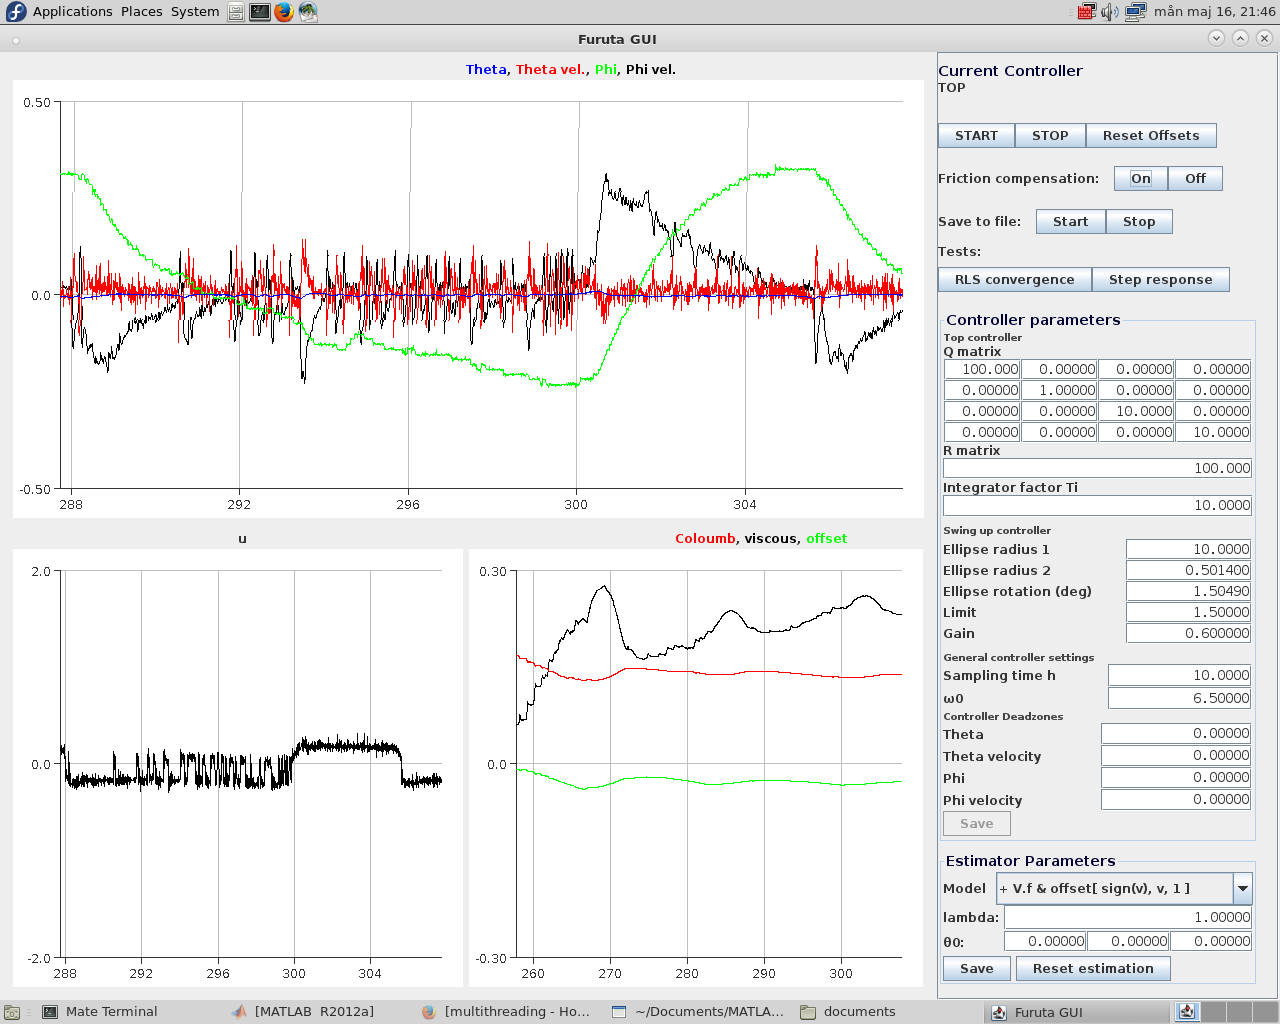
\includegraphics[scale=0.4]{gui.png}}
\caption{Suggested design for the GUI}
\label{fig:uml}
\end{figure}
\section{Time plan}
\begin{table}[H]
\centering
\caption{Time plan}
\label{hoho}
\begin{tabular}{|l|l|l|}
\hline
Week & Description & Main Responsibility \\ \hline
13 & Hand in project plan & All members \\ \hline
& Begin GUI implementation & Adam \\ \hline
& Begin implementation of Java controller & Alexander \\ \hline
& Begin implementation of Matlab controller & Jonathan \\ \hline
& Research on friction estimator and model & Jonathan \\ \hline
14 & Working GUI implementation & Adam \\ \hline
& Write skeleton for report & Emil \\ \hline
& Working basic implementation of Java controller & Alexander \\ \hline
& Working basic implementation of Matlab controller & Jonathan \\ \hline
15 & Finished Matlab controller for tests & Jonathan \\ \hline
& Predictive theory complete  & Emil \\ \hline
& All code complete, begin testing and tuning & All members \\ \hline
16 & Begin Predictive presentation & Alexander \\ \hline
& Realtime theory complete & Adam \\ \hline
17 & Predictive presentation 29/4 & \\ \hline
18 & Adapt presentation for Realtime course & Jonathan \\ \hline
19 & Fine tune until perfection & All Members \\ \hline
20 & Realtime presentation 19/5  & \\ \hline
\end{tabular}
\end{table}
The aim is to finish the GUI as soon as possible to be able to properly evaluate our controller. The controller will first be done in Matlab since a working solution already exist except for the RLS estimator. This also makes it easier to evaluate the controller in Java since the expected behavior is then known.

The report will be written concurrently to the work on the other parts.




\section{Responsibilities}
\begin{itemize}
\item Theory - Emil
\item Report - Emil
%	What estimators to use\\
%	What friction model
\item Friction controller in MATLAB - Jonathan
\item Controller in Java - Alexander
%	Friction\\
%	Swingup\\
%	Top controller
\item GUI - Adam
\item Presentation - Jonathan

\end{itemize}


\end{document}

